\chapter{Background}
\label{ch:background}

In this chapter, we begin by providing a comprehensive overview of the CUDA programming model and GPU microarchitecture, 
ensuring that readers have a solid understanding of the key concepts and components that define the CUDA 
ecosystem. Next, we introduce the MWP-CWP analytical model, which sheds light on the parallelism exhibited 
by Memory Warp Parallelism (MWP) and Computation Warp Parallelism (CWP) in GPU architectures. This model 
plays a critical role in analyzing and optimizing the performance of CUDA kernels. Through a clear explanation 
of these fundamental concepts, this chapter sets the stage for a deeper exploration of KLARAPTOR and its application 
in enhancing the performance of CUDA programs.

\section{CUDA}
\label{sec:cuda}

In this section, a concise introduction to Compute Unified Device Architecture (CUDA) is presented. 
CUDA, designed by NVIDIA, is a heterogeneous serial-parallel programming model\cite{marcmwpcwpslides} that capitalizes on 
the capabilities of GPUs for general-purpose computation. Primarily 
targeting C/C++ programmers, CUDA has revolutionized the field of high-performance computing by 
facilitating substantial performance enhancements across various domains, including scientific 
simulations, artificial intelligence, and more. This background information aims to provide the 
foundations for comprehending the fundamental concepts, techniques, and challenges associated with 
GPU-accelerated computation.\cite{cuda2016best}

\subsection{Graphics Processing Unit (GPU)}
\label{sec:gpu}
A GPU is a specialized computational device designed for quick manipulation and alteration of memory, 
primarily to generate images for display on a screen. Initially, GPUs were mainly used for rendering 3D graphics in video games 
and other visually intensive applications. However, their highly parallel structure and ability to process large amounts of data 
simultaneously have made them increasingly valuable for general-purpose computation tasks.

Within the realm of CUDA programming, a GPU serves as a powerful computational device capable of executing thousands of threads in 
parallel. This allows it to perform complex calculations and data processing at a much faster rate than traditional Central Processing 
Units (CPUs), which focus on executing a smaller number of threads rapidly. By understanding the architecture and capabilities of GPUs, 
developers can utilize the CUDA programming model effectively to harness their computational power for various applications beyond 
graphics rendering.

The relevance of GPUs to the CUDA programming model lies in their ability to significantly enhance the 
performance of parallel computation. CUDA exploits the inherent advantages of GPUs to facilitate 
general-purpose computation on these devices, effectively transforming them into potent computational 
tools beyond their conventional graphics rendering roles\cite{cuda2016best}.

GPUs offer substantial advantages over CPUs in the context of instruction throughput and memory bandwidth, 
while maintaining comparable costs and power consumption. This is primarily due to the distinct design 
goals of GPUs and CPUs. Mentioned above, CPUs focus on executing a few tens of threads rapidly, while GPUs are engineered 
to excel at executing thousands of threads in parallel, compensating for slower single-thread performance 
to achieve greater overall throughput. Figure~\ref{fig:gpuvscpu} shows the distribution of chip resources 
for a CPU versus a GPU.

\begin{figure}[htb]
    \centering
    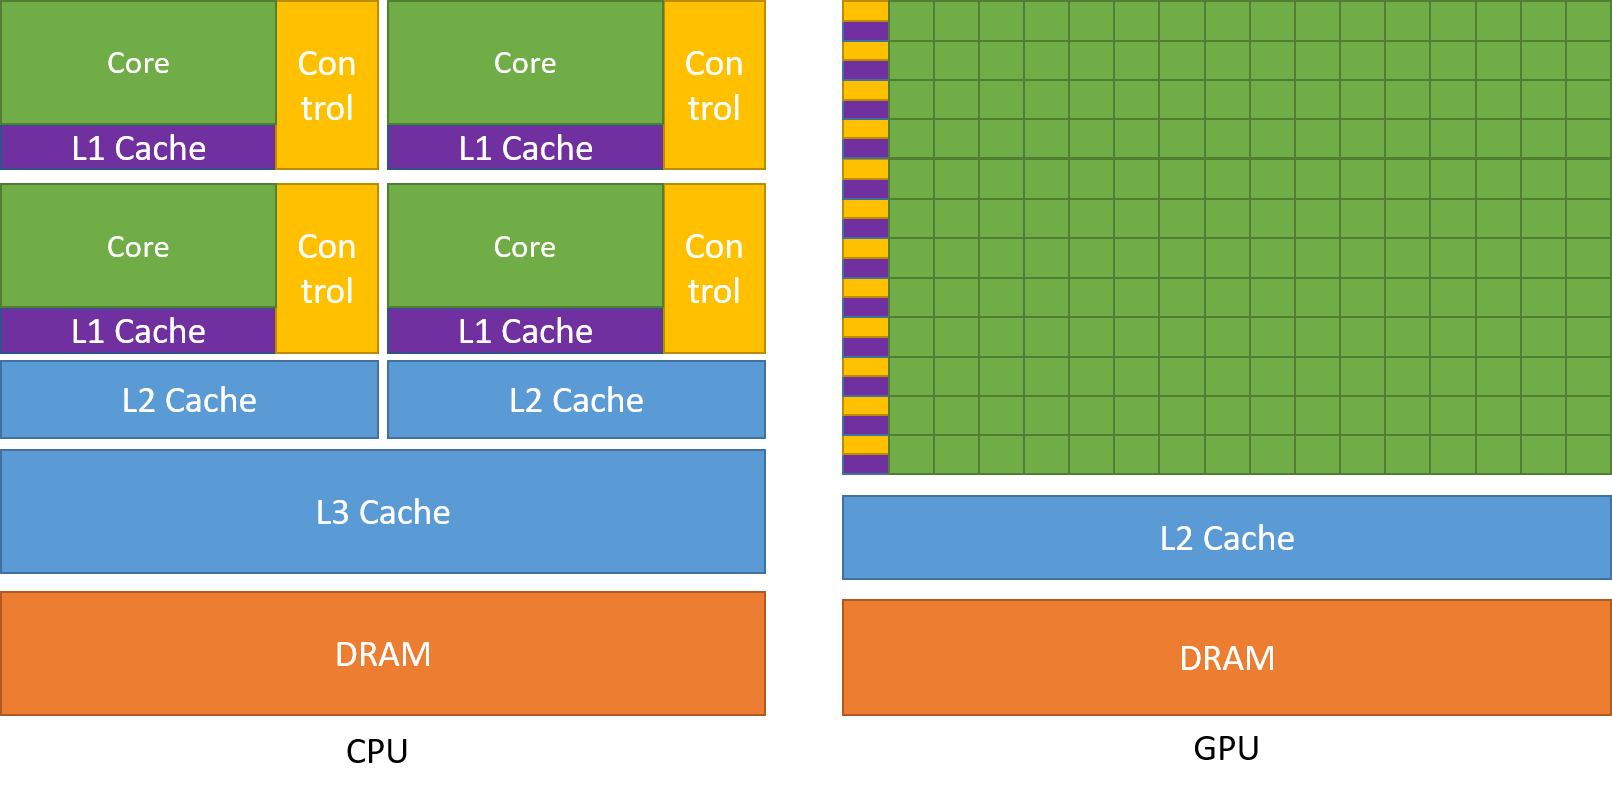
\includegraphics[width=0.65\linewidth]{Figures/gpu-devotes-more-transistors-to-data-processing.png}
	\caption{The GPU Devotes More Transistors to Data Processing}
	\label{fig:gpuvscpu}
\end{figure}

\subsection{CUDA Programming Model}
\label{sec:cudapromodel}
The CUDA parallel programming model addresses the challenges of scalable parallelism\cite{marccudaslides} while retaining 
accessibility for programmers familiar with languages such as C/C++. At the core of this model lie three 
fundamental abstractions—hierarchy of thread groups, shared memories, and barrier 
synchronization—introduced as minimal language extensions. These abstractions enable a combination of 
fine-grained and coarse-grained parallelism, directing programmers to partition problems into independently 
solvable sub-problems and fostering cooperative parallel problem-solving within thread blocks. 
This methodology not only maintains language expressivity but also permits automatic scalability, as each 
thread block can be scheduled on any accessible GPU multiprocessor, with the runtime system overseeing 
the physical multiprocessor count\cite{cuda2016best}. Figure~\ref{fig:cpuvsgpupro} shows an example of a CPU program vs a CUDA program.

\begin{figure}[htb]
    \centering
    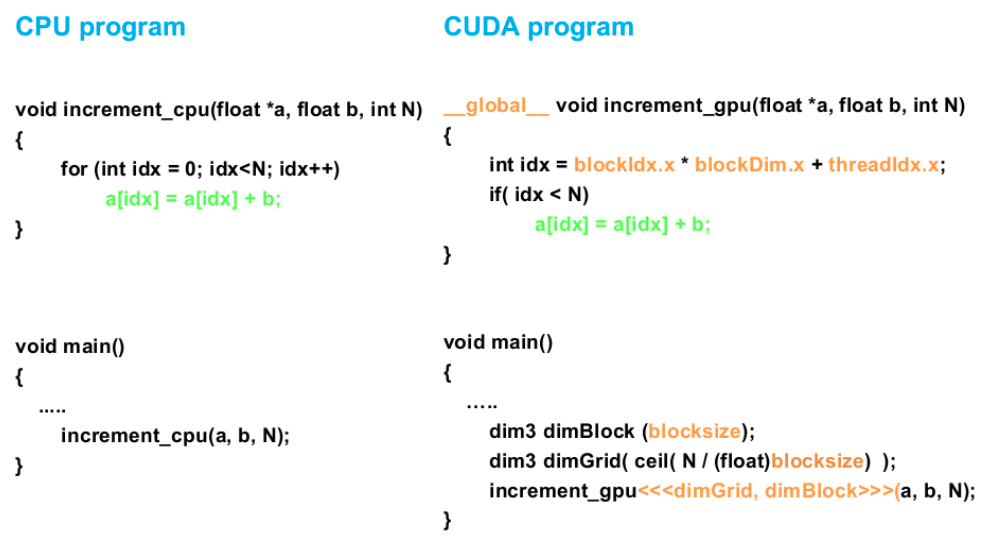
\includegraphics[width=0.85\linewidth]{Figures/CPUvsGPUprogram.png}
    \caption{Example of a CPU program vs a CUDA program}
    \label{fig:cpuvsgpupro}
\end{figure}

\subsubsection{Kernels}
\label{sec:kernels}
CUDA kernels are the fundamental building blocks of a CUDA program, representing the functions 
that execute on the GPU device (also referred to as the device) in parallel. In the context of 
CUDA, the CPU is referred to as the host, responsible for managing and orchestrating the execution 
of kernels on the device\cite{marccudaslides}. The device is typically composed of multiple streaming multiprocessors 
(SMs) that provide the parallel processing capability. A kernel is defined in the CUDA programming 
model using the \mintinline{cuda}{__global__} declaration specifier, which indicates that the function is callable 
from the host and executes on the device. The execution configuration of a kernel is specified 
using \mintinline{cuda}{<<<...>>>}, which determines the grid and block dimensions, 
thereby dictating the number of parallel threads and their organization during kernel execution\cite{cuda2016best}. 
This configuration allows programmers to efficiently utilize the available resources on the GPU 
and optimize the performance of their CUDA applications.

\subsubsection{Threads}
\label{sec:threads}
In the CUDA programming model, threads constitute the basic units of parallel execution and are 
organized within a hierarchical structure encompassing threads, thread blocks, and grids. Each 
thread is uniquely identified by its \mintinline{cuda}{threadIdx}, which is a multi-dimensional variable with up to 
three dimensions (x, y, and z)\cite{cuda2016best}. Thread limits are dictated by the GPU architecture, with the 
maximum number of threads per block typically capped at 1024. Threads are assembled into blocks, 
which are then organized into a grid. The \mintinline{cuda}{blockIdx} and \mintinline{cuda}{blockDim} variables identify the position 
of a specific block within the grid and the dimensions of each block, respectively. Thread and 
block dimensions can be one-, two-, or three-dimensional, offering flexibility in addressing the 
problem space in a manner that best accommodates the underlying data structure and computation. 
This hierarchical organization of threads and blocks enables efficient mapping of intricate, 
multi-dimensional problems onto the GPU's parallel processing resources, promoting optimal 
performance and resource utilization.

Thread blocks hold a pivotal role in the CUDA programming model\cite{marccudaslides}, functioning as a means to 
organize threads that collaboratively work on a specific sub-problem. Within a thread block, 
threads can communicate and synchronize their operations via shared memory, facilitating efficient 
data exchange and cooperative problem-solving. It is important to note that thread blocks can be 
executed in any order, both concurrently and sequentially, across the available SMs on a GPU. This 
flexibility permits automatic scalability, allowing the compiled CUDA program to adapt to varying 
GPU architectures and multiprocessor counts\cite{cuda2016best}. Consequently, thread blocks enable efficient utilization 
of GPU resources while ensuring that applications can scale effectively on diverse hardware configurations.

\subsubsection{Kernel Launch Parameters}
\label{sec:kernellaunchparameters}

When launching a CUDA kernel, the execution configuration specified plays a crucial role in determining 
the organization of threads and blocks for the kernel's execution on the GPU. The launch parameters 
within this syntax define the grid and block dimensions, which impact the performance and resource 
utilization of the application.

The launch parameters consist of two main components: the number of blocks per grid (\mintinline{cuda}{gridDim}) and the 
number of threads per block (\mintinline{cuda}{blockDim}). Both of these parameters can be specified as one-, two-, or 
three-dimensional structures, represented by dim3 variables in CUDA. The choice of dimensions depends 
on the problem space and the structure of the underlying data, with the aim of efficiently mapping the 
computation onto the GPU's resources.

For example, if a kernel is launched with the configuration \mintinline{cuda}{<<<gridDim, blockDim>>>}, it will create 
$gridDim.x * gridDim.y * gridDim.z$ blocks in the grid, with each block 
containing $blockDim.x * blockDim.y * blockDim.z$ threads. This results in a total of 
$(gridDim.x * gridDim.y * gridDim.z) * (blockDim.x * blockDim.y * blockDim.z)$ threads executing the 
kernel concurrently.

Selecting optimal launch parameters is essential for achieving maximum performance and resource 
utilization on the GPU\cite{cuda2019guide}. The choice of grid and block dimensions should consider factors such as the 
size of the problem, the hardware limitations of the GPU (e.g., maximum threads per block), and the 
level of parallelism required. Additionally, it is important to account for shared memory constraints, 
as larger block sizes may lead to increased shared memory requirements, potentially causing resource 
allocation issues or reduced parallelism\cite{cuda2019guide}.

By carefully choosing the launch parameters for a CUDA kernel, developers can create efficient, 
high-performance parallel applications that effectively exploit the capabilities of the underlying GPU hardware.\cite{cuda2019guide}

\subsection{CUDA by Example}
\label{sec:cudabyexample}

In the following section, we shall explore a fundamental example of CUDA programming by implementing a vector 
addition program. This hands-on approach will enable readers to gain a deeper understanding of the various components 
and concepts involved in writing and executing CUDA code. This example follows a GitHub repository, If you would like 
to explore this tutorial further and experiment with the code, it is available at the following \cite{Papatheodore2022}.

\definecolor{LightGray}{gray}{0.9}
\begin{minted}
[
frame=lines,
framesep=2mm,
baselinestretch=0.75,
bgcolor=LightGray,
fontsize=\footnotesize,
linenos,
samepage
]
{cuda}
#include <stdio.h>

// Size of array
#define N 1048576

// Kernel
__global__ void add_vectors(double *a, double *b, double *c)
{
	int id = blockDim.x * blockIdx.x + threadIdx.x;
	if(id < N) c[id] = a[id] + b[id];
}

// Main program
int main()
{
	// Number of bytes to allocate for N doubles
	size_t bytes = N*sizeof(double);

	// Allocate memory for arrays A, B, and C on host
	double *A = (double*)malloc(bytes);
	double *B = (double*)malloc(bytes);
	double *C = (double*)malloc(bytes);

	// Allocate memory for arrays d_A, d_B, and d_C on device
	double *d_A, *d_B, *d_C;
	cudaMalloc(&d_A, bytes);
	cudaMalloc(&d_B, bytes);
	cudaMalloc(&d_C, bytes);

	// Fill host arrays A and B
	for(int i=0; i<N; i++)
	{
		A[i] = 1.0;
		B[i] = 2.0;
	}

	// Copy data from host arrays A and B to device arrays d_A and d_B
	cudaMemcpy(d_A, A, bytes, cudaMemcpyHostToDevice);
	cudaMemcpy(d_B, B, bytes, cudaMemcpyHostToDevice);

	// Set execution configuration parameters
	//		thr_per_blk: number of CUDA threads per grid block
	//		blk_in_grid: number of blocks in grid
	int thr_per_blk = 256;
	int blk_in_grid = ceil( float(N) / thr_per_blk );

	// Launch kernel
	add_vectors<<< blk_in_grid, thr_per_blk >>>(d_A, d_B, d_C);

	// Copy data from device array d_C to host array C
	cudaMemcpy(C, d_C, bytes, cudaMemcpyDeviceToHost);

	// Free CPU memory
	free(A);
	free(B);
	free(C);

	// Free GPU memory
	cudaFree(d_A);
	cudaFree(d_B);
	cudaFree(d_C);

	return 0;
}
\end{minted}

\addvspace{5cm}

We initiate the process at line 17, where the memory requirement for an array comprising N double-precision elements is 
determined. Subsequently, memory allocation for vectors A, B, and C occurs on the host in lines 20-22. Continuing forward, 
lines 25-28 allocate memory on the device for the same vectors. It is worth noting the prevalent naming convention for device 
variables is ``d\_'' prefix to indicate device allocation.

The host input vectors A and B are copied to their device counterparts, d\_A and d\_B with \mintinline{cuda}{cudaMemcpy()} 
as seen in lines 38-39. To prepare for kernel 
launch, we set the kernel launch parameters in lines 44-45, defining the number of threads per block and the number of 
blocks per grid. The kernel is then launched in line 48, where the actual computation is executed.

Focusing on the \mintinline{cuda}{add_vectors} kernel function at line 7, a unique thread ID is identified in line 9 
for each thread within 
the grid. The \mintinline{cuda}{if} statement on line 10 serves to prevent memory access beyond the array's bounds, 
which may occur when 
the number of grid threads is not a multiple of the number of threads per block. For instance, if N has an extra element, 
\mintinline{cuda}{blk_in_grid} would equal 4097 due to the \mintinline{cuda}{ceil} function in line 45, resulting in a total of 
$4097*256 = 1048832$ threads. 
Without the \mintinline{cuda}{if} statement, the final thread would attempt to access memory beyond the array's boundaries.

In conclusion, the device output vector d\_C is copied to the host output vector C in line 51. Host memory is then freed 
in lines 54-56, followed by the release of device memory in lines 59-61.

\begin{figure}[htb]
    \centering
    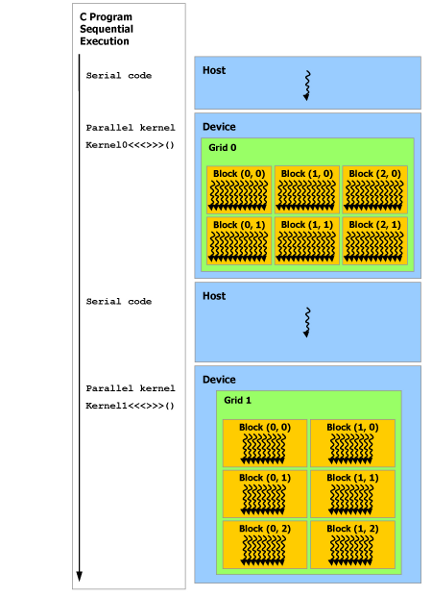
\includegraphics[width=0.65\linewidth]{Figures/heterogeneous-programming.png}
	\caption{Heterogeneous Programming Model for CUDA}
	\label{fig:heteropro}
\end{figure}

\subsection{CUDA Memory Model}
\label{sec:cudamemmodel}

\begin{figure}[htb]
    \centering
    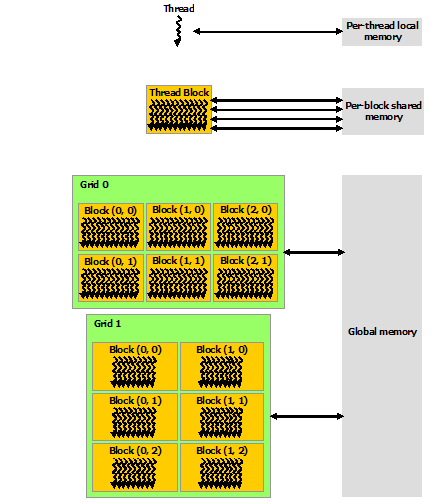
\includegraphics[width=0.65\linewidth]{Figures/memory-hierarchy.png}
	\caption{CUDA Memory Hierarchy}
	\label{fig:memhierarchy}
\end{figure}

The CUDA memory model is designed to accommodate the unique requirements of parallel programming 
on GPUs and consists of several distinct memory spaces. Host memory refers to the system memory 
allocated and managed by the CPU. In contrast, the GPU has its own memory spaces, including global, 
shared, and local memory\cite{cuda2016best}.

Global memory, accessible by all threads within a kernel as well as the host, serves as the primary 
means for data storage and communication between the host and the device. The lifetime of data in global 
memory spans from the point of allocation to deallocation, which is explicitly managed by the programmer. 
Although global memory offers a large storage capacity, it has higher access latency compared to other 
memory spaces on the GPU\cite{cuda2016best}.

Shared memory, as the name suggests, is a fast, on-chip memory space that can be shared among threads 
within the same thread block. This memory space enables efficient inter-thread communication and data 
exchange, making it particularly useful for problems that require threads to cooperate and share 
information while solving sub-problems. However, shared memory is limited in capacity, and its contents 
are only available for the duration of a thread block's execution\cite{cuda2016best}.

Local memory is private to each individual thread and is used for storing thread-specific data, such as 
function call frames and automatic variables. While local memory is accessible only by the thread that 
owns it, it allows threads to store temporary data without affecting other threads. Similar to global memory, 
local memory resides off-chip, and therefore, its access latency is higher than that of shared memory.

Refer to Figure~\ref{fig:memhierarchy} for a visual representation of the CUDA memory hierarchy.

\subsection{GPU Microarchitecture}
\label{sec:gpumicroarchitecture}

We introduce the fundamental concepts of GPU microarchitecture, highlighting their 
relation to the CUDA programming model\cite{cuda2016best}. Understanding these core principles allows for a deeper 
comprehension of the efficient execution of parallel workloads on GPUs and informs the development 
of effective CUDA applications.

\subsubsection{SIMT and SIMD}
\label{sec:simdandsimt}

SIMT (Single Instruction, Multiple Thread) and SIMD (Single Instruction, Multiple Data) 
constitute vital parallel execution models that impact the performance of GPU architectures
and their integration with the CUDA programming model. SIMT operates by executing identical 
instructions on distinct threads, while SIMD conducts the same operation on multiple data elements. 
NVIDIA GPUs utilize the SIMT paradigm, permitting threads to be organized into warps that 
execute instructions concurrently, thus optimizing resource usage and reducing thread management 
overhead\cite{cuda2016best}. The CUDA programming model corresponds directly to the SIMT architecture, empowering developers 
to harness the inherent parallelism of GPUs while efficiently handling threads, memory, and 
synchronization to achieve exceptional parallel computing performance.

\subsubsection{Streaming Multiprocessors (SMs)}
\label{sec:sm}

Streaming Multiprocessors (SMs) are the primary building blocks of NVIDIA GPUs, acting as the core 
computational units that enable efficient parallel processing. Each SM houses multiple execution 
units, registers, and shared memory, facilitating the concurrent execution of a large number of threads. 
In CUDA, developers organize threads into blocks, which are then scheduled onto SMs\cite{cuda2016best}. This arrangement 
allows for effective management of thread parallelism, memory, and synchronization, ensuring optimal GPU 
resource utilization and high-performance parallel computing.

\subsubsection{Warp and Warp Scheduling}
\label{sec:warp}

Warps and warp scheduling are essential components of GPU architectures, particularly in the context 
of CUDA programming. In CUDA, a warp is a group of threads, typically 32, that execute simultaneously 
on a single streaming multiprocessor (SM). Threads within a warp share a common program counter and 
follow a simultaneous execution pattern, optimizing resource utilization and reducing thread management 
overhead. Warp scheduling, on the other hand, is instrumental in managing how warps execute on SMs. 
Different GPU architectures use various scheduling policies, determining the selection and instruction 
issuance for ready warps\cite{cuda2016best}. Efficient warp scheduling is crucial for maximizing GPU resource utilization 
and overall performance.


\section{MWP-CWP}
\label{sec:mwp-cwp}

The MWP-CWP analytical model offers a novel approach to understanding the performance of GPU 
architectures by examining the parallelism exhibited by MWP and CWP. As multithreaded architectures, GPUs allow multiple warps 
to be executed concurrently on a streaming multiprocessor (SM), effectively hiding the execution 
costs of these warps. The MWP-CWP model focuses on determining the maximum number of warps that 
can access memory simultaneously and the number of warps that an SM processor can execute during 
a memory warp waiting period. By carefully analyzing the relationship between MWP and CWP, this 
model provides valuable insights into the factors that govern execution time, revealing whether 
it is dominated by computation or memory access costs. Through a series of illustrative cases, we 
will demonstrate the importance of sufficient warps and the intricate interplay between MWP and CWP 
in optimizing GPU performance.\cite{DBLP:conf/isca/HongK09,marcmwpcwpslides}

\begin{figure}[H]
	\centering % <-- added
	\begin{subfigure}[b]{0.55\textwidth}
        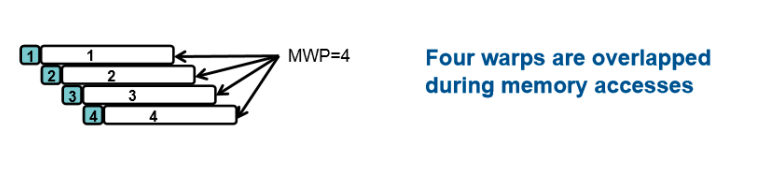
\includegraphics[width=\linewidth]{Figures/MWP.png}
        \caption{MWP}
        \label{fig:mwp}
	\end{subfigure}\hfil % <-- added
	\begin{subfigure}[b]{0.45\textwidth}
		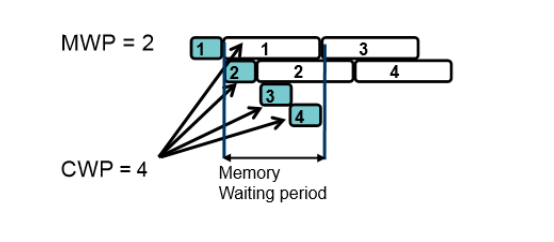
\includegraphics[width=\linewidth]{Figures/CWP.png}
	    \caption{CWP}
	    \label{fig:cwp}
	\end{subfigure}
	\label{fig:mwpcwpmodel}
    \caption{MWP-CWP model}
\end{figure}

\subsection{$MWP \leq CWP$}
\label{sec:mwp-cwp:1}

In the case where CWP is greater than MWP, the application's performance exhibits a distinct 
characteristic: computation cycles are effectively hidden by memory waiting periods. This implies 
that the computational resources are kept busy while the memory accesses are being processed, 
leading to a more efficient use of the available resources. However, the overall performance of 
the application is dominated by the memory cycles, as the computational work is executed in parallel 
with memory access operations. In other words, the system exhibits a higher degree of parallelism in 
computation than in-memory operations. This implies that while the application effectively utilizes 
the available computational resources, it may face limitations in leveraging memory-level parallelism. 
This imbalance between CWP and MWP can result in the underutilization of memory bandwidth and potentially 
lead to performance bottlenecks.\cite{DBLP:conf/isca/HongK09,marcmwpcwpslides}

\begin{figure}[htb]
    \centering
    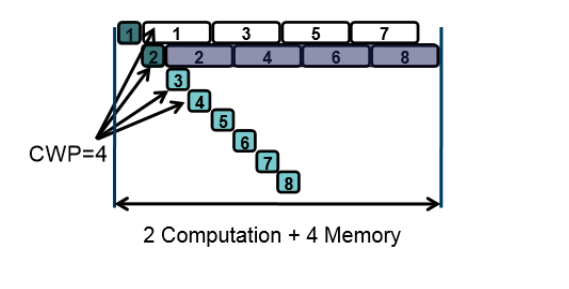
\includegraphics[width=0.65\linewidth]{Figures/cwpgreaterthanmwp.png}
	\caption{Computation cycles are concealed by memory waiting periods, 
             resulting in the overall performance being predominantly dictated by memory cycles.}
	\label{fig:cwpgreaterthanmwp}
\end{figure}

\subsection{$MWP > CWP$}
\label{sec:mwp-cwp:2}

In the scenario where MWP is greater than CWP, the application's performance demonstrates a contrasting behavior: 
memory accesses are predominantly hidden due to the high MWP. This means that the memory subsystem is capable 
of handling multiple memory requests concurrently while the computation resources are being utilized, 
effectively masking memory latencies. As a result, the overall performance of the application is dominated 
by the computation cycles, since the memory accesses are efficiently processed in parallel with the computational 
work. To put it differently, the application's performance may be hindered due to an imbalance between memory 
and computational resources. This disparity indicates that the application has a higher degree of parallelism 
in memory access than in computation, which can potentially result in the underutilization of computational 
resources.\cite{DBLP:conf/isca/HongK09,marcmwpcwpslides}

\begin{figure}[htb]
    \centering
    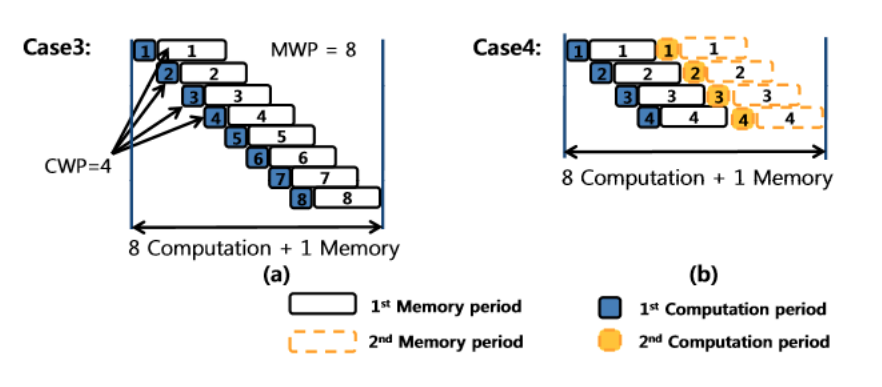
\includegraphics[width=0.65\linewidth]{Figures/mwpgreaterthancwp.png}
	\caption{Memory accesses are largely concealed by high MWP, 
            leading to the overall performance being primarily governed by computation cycles.}
	\label{fig:mwpgreaterthancwp}
\end{figure}




